\documentclass[screen]{beamer}
\usepackage[T1]{fontenc}
\usepackage[latin1]{inputenc}
\usepackage{amsmath}
\usepackage{bm}



% Bruk NTNU-temaet for beamer (her i bokmålvariant), alternativer er
% ntnunynorsk og ntnuenglish.
\usetheme{ntnuenglish}
 
% Angi tittelen, vi gir også en kortere variant som brukes nederst på
% hver slide:
\title[The Finite Element Method]%
{Bake, Shake or Break: \\Breaking a wooden bridge}

% Denne kan du også bruke hvis det passer seg:
%\subtitle{Valgfri undertittel}

% Angir foredragsholder, også en (valgfri) kortversjon i
% hakeparanteser først som kommer nederst på hver slide:
\author[Halvorsen \& Hasund]{Halvorsen \& Hasund}

% Institusjon. Bruk gjerne disse slik det passer best med det du vil
% ha.  Valgfri kortversjon her også
\institute[NTNU]{The Finite Element Method project}

% Datoen blir også trykket på forsida. 
\date{16. November 2014}
%\date{} % Bruk denne hvis du ikke vil ha noe dato på forsida.

% Fra her av begynner selve dokumentet
\begin{document}
\setbeamertemplate{itemize items}[circle]

% Siden NTNU-malen har en annen bakgrunn på forsida, må dette gjøres
% i en egen kommando, ikke på vanlig beamer-måte:
\ntnutitlepage

% Her begynner første slide/frame, (nummer to etter forsida). 

\begin{frame}
\frametitle{Motivation}

 Sydney Harbour bridge
\begin{columns}   
    \begin{column}{.5\linewidth}
        \begin{figure}
  		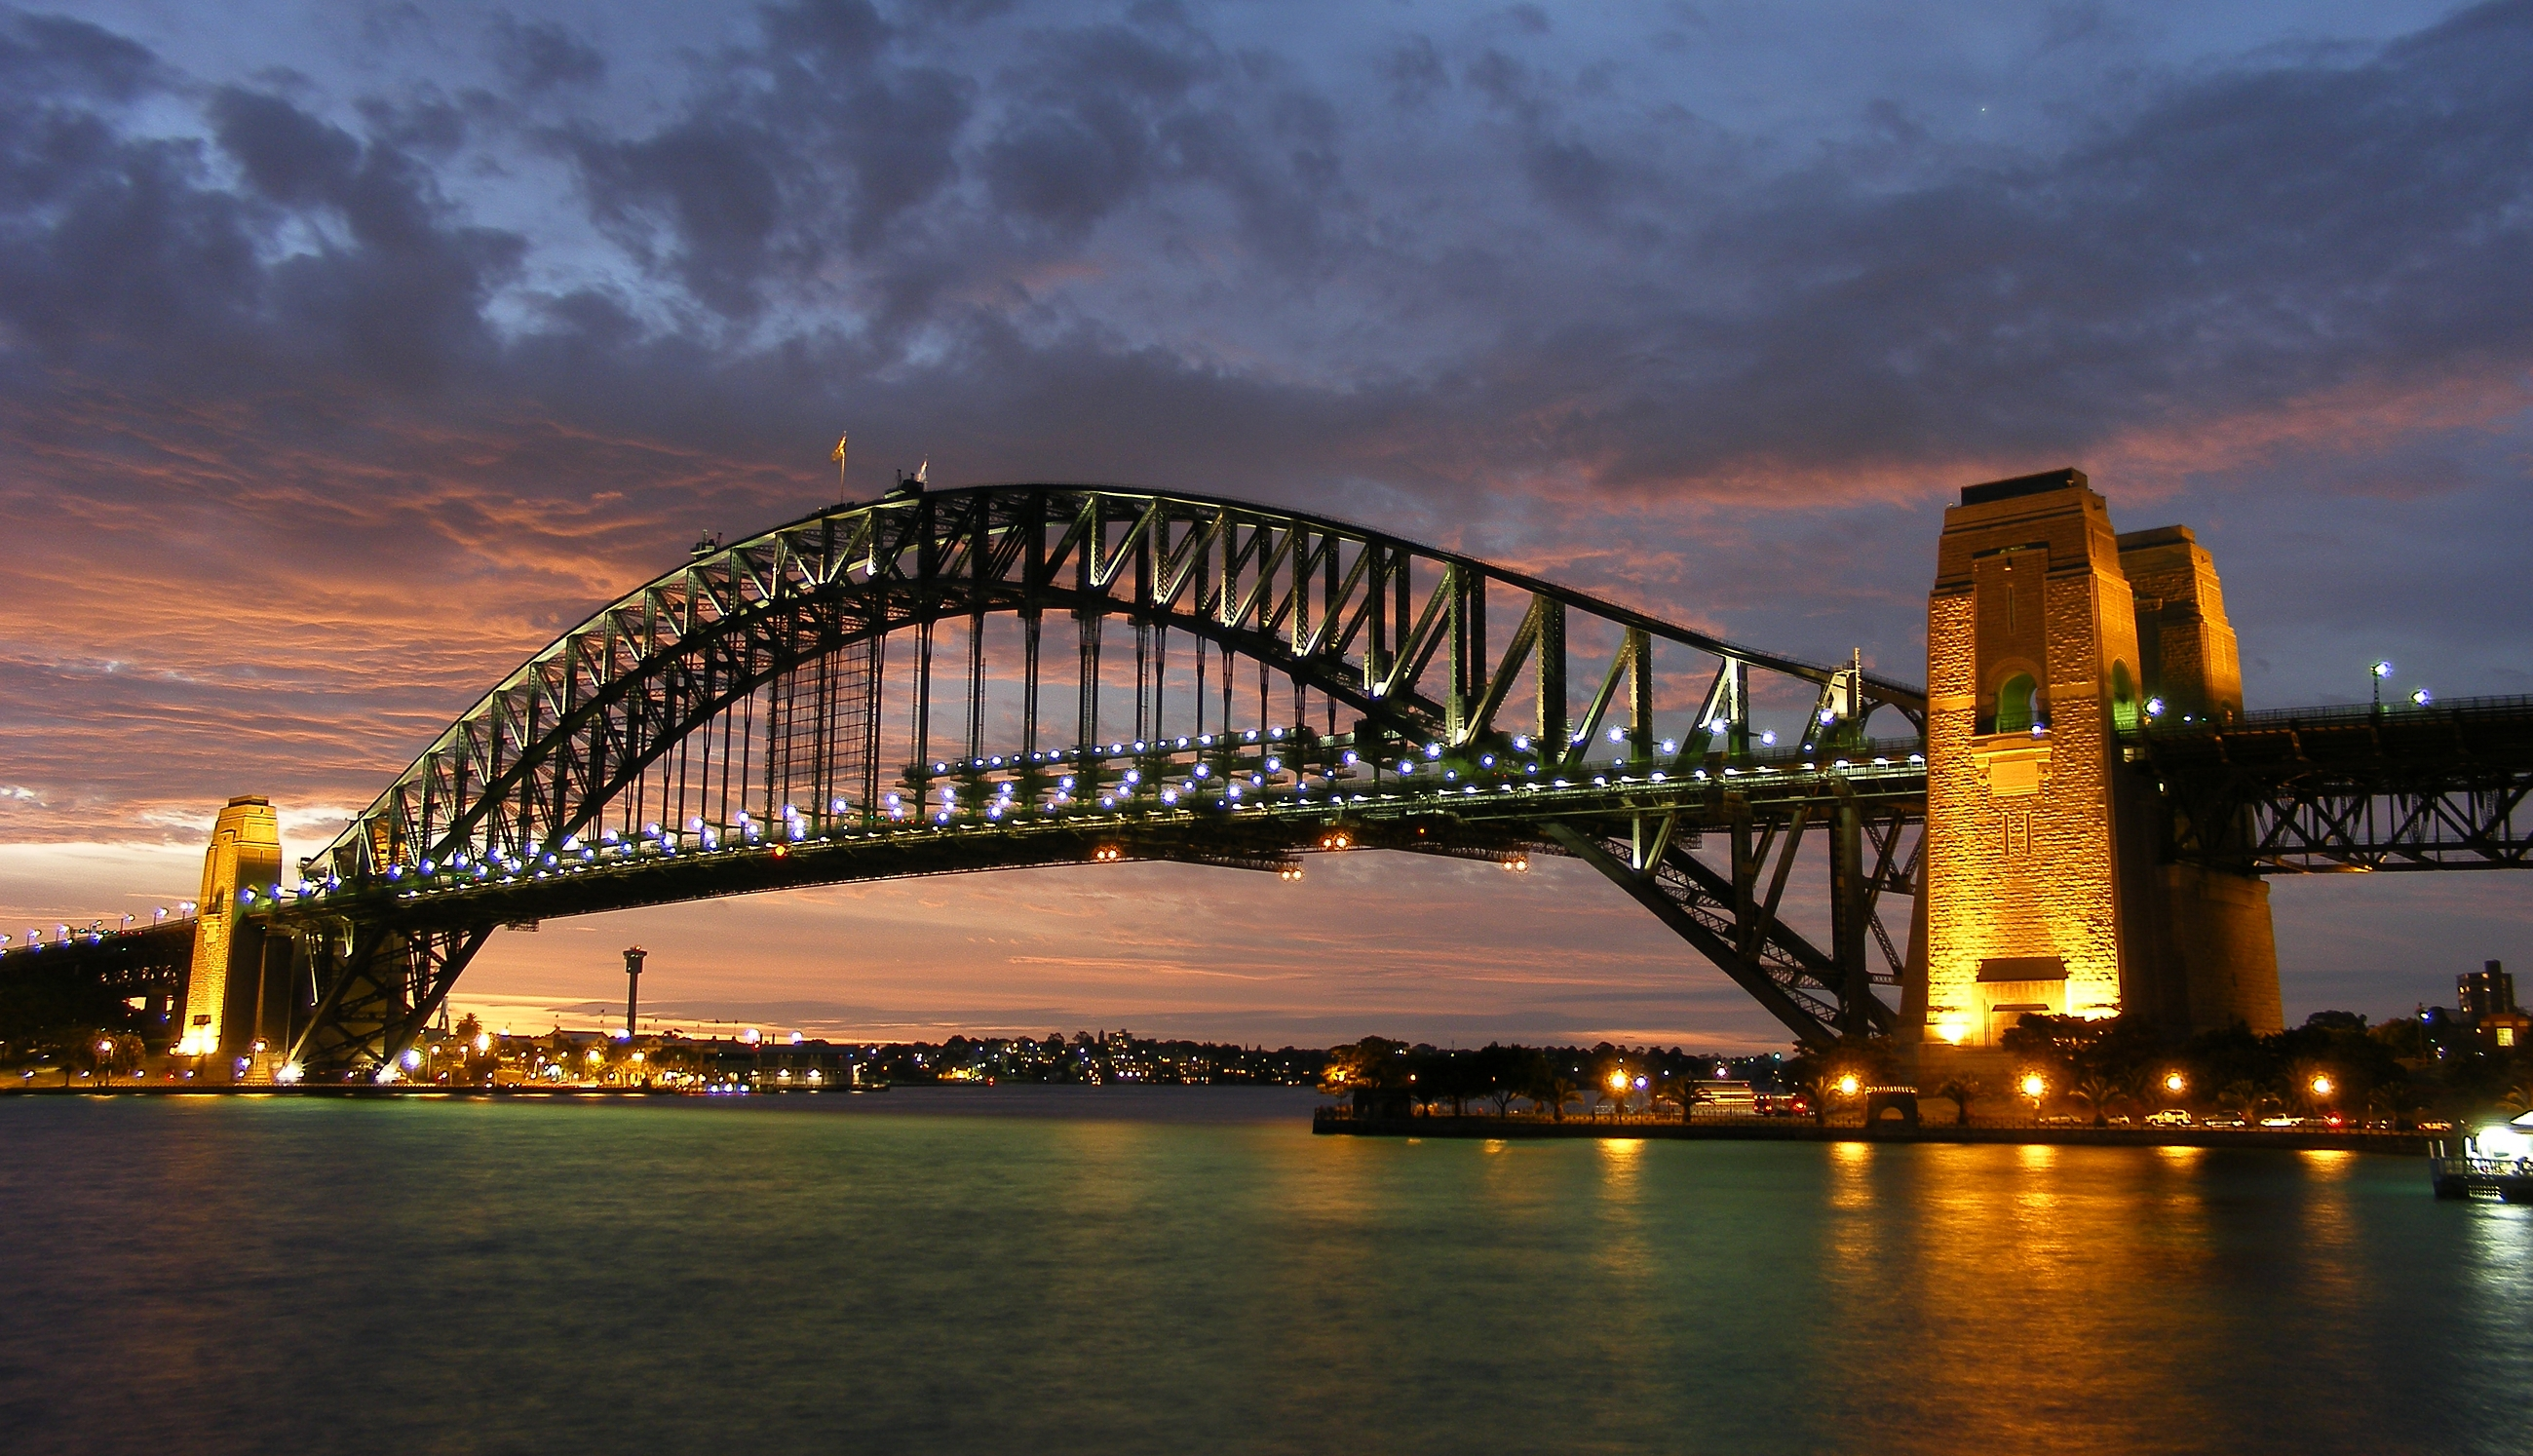
\includegraphics[scale=0.25]{figures/Sydney_pic}
  		\end{figure}
    \end{column}   
    \begin{column}{.5\linewidth}

        \begin{figure}
  		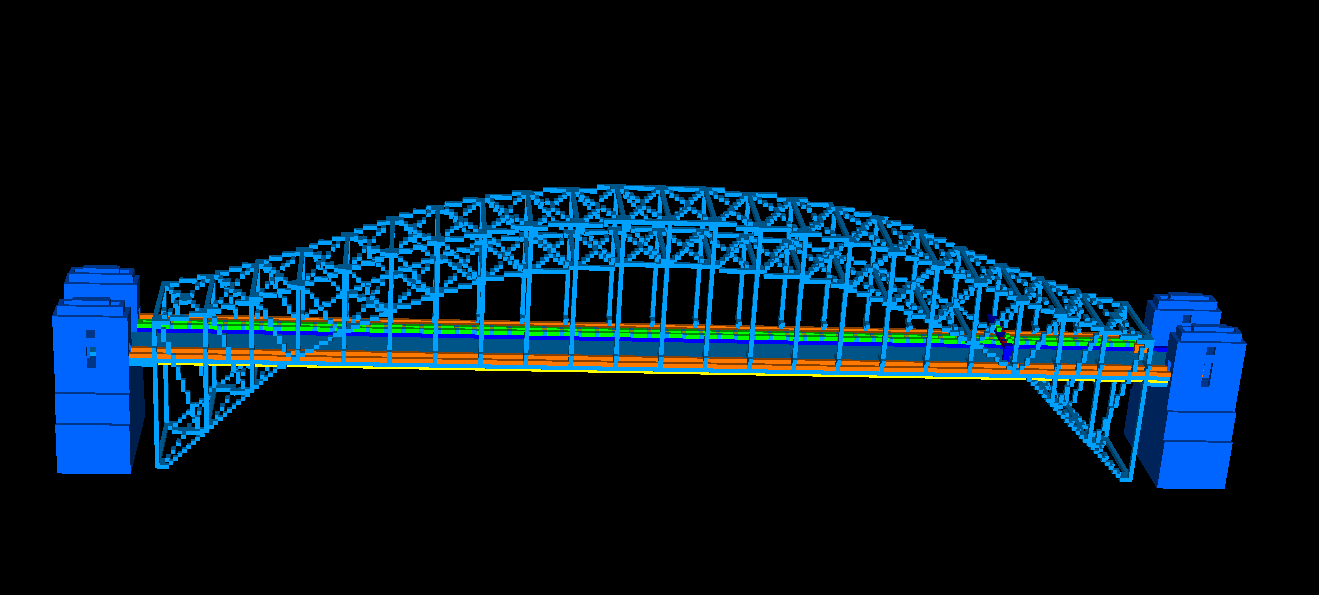
\includegraphics[scale=0.12]{figures/sydneyBridge}
  		\end{figure}
    \end{column}
  \end{columns}
\end{frame}

\begin{frame}
\begin{columns}
    \begin{column}{\linewidth}
      \begin{block}{Linear Elasticity Equation}
         \begin{align*}
         \nabla \sigma(u) = -f
         \end{align*}
         \begin{itemize}
         \centering
         \item[$\sigma$: ] stress
         \item[$u$: ] displacement
         \item[$f$: ] force
         \item[ ]
         \end{itemize}
      \end{block}
    \end{column}
  \end{columns}
\end{frame}

\begin{frame}
2D model

	\begin{align*}
	f_x = \frac{E}{1-\nu^2} (-2y^2 - x^2 + \nu x^2 - 2\nu xy -2xy + 3 - \nu) \\
	f_y = \frac{E}{1-\nu^2} (-2x^2 - y^2 + \nu y^2 - 2\nu xy -2xy + 3 - \nu) 
	\end{align*}
\end{frame}

\begin{frame}
Error and convergence


\begin{columns}   
    \begin{column}{.5\linewidth}
        \begin{figure}
  		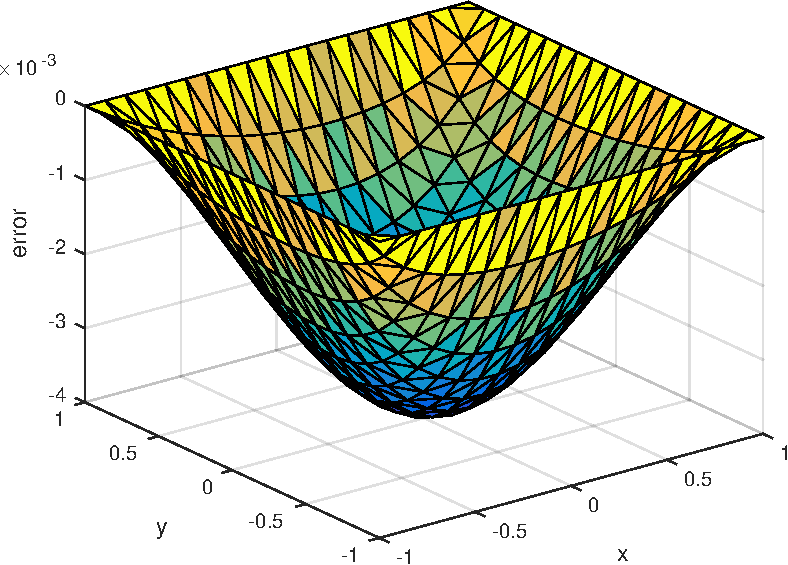
\includegraphics[scale=0.35]{figures/error_linEl}
  		\end{figure}
    \end{column}   
    \begin{column}{.5\linewidth}

        \begin{figure}
  		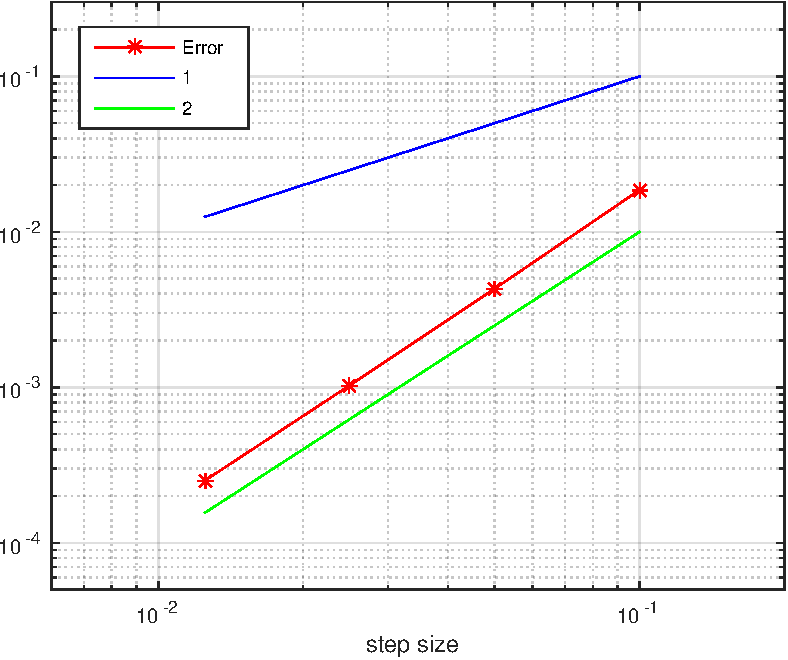
\includegraphics[scale=0.35]{figures/conv_linEl}
  		\end{figure}
    \end{column}
  \end{columns}

\end{frame}

\begin{frame}
\frametitle{Linear Elasticity Problem in 3D}
\begin{align*}
\begin{bmatrix}
\frac{\partial}{\partial x}, & \frac{\partial}{\partial y}, & \frac{\partial}{\partial z}
\end{bmatrix}
\begin{bmatrix}
\sigma_{xx} & \sigma_{xy} & \sigma_{xz} \\
\sigma_{xy} & \sigma_{yy} & \sigma_{yz} \\
\sigma_{xz} & \sigma_{yz} & \sigma_{zz}
\end{bmatrix} = -
\begin{bmatrix}
f_x, & f_y, & f_z 
\end{bmatrix}.
\end{align*}
\end{frame}

\begin{frame}
Relation between stress and displacement
\begin{align*}
\sigma = C B u
\end{align*}
\tiny
\begin{align*}
u &= 
\begin{bmatrix}
u_{1_x}, u_{1_y}, u_{1_z}, &...&  u_{4_x}, u_{4_y}, u_{4_z}
\end{bmatrix}^T  \\
{\sigma} &=
\begin{bmatrix}
\sigma_{xx} \\
\sigma_{yy} \\
\sigma_{zz} \\
\sigma_{xy} \\
\sigma_{yz} \\
\sigma_{xz}
\end{bmatrix}, \,
{\epsilon} = 
\begin{bmatrix}
\epsilon_{xx} \\
\epsilon_{yy} \\
\epsilon_{zz} \\
\epsilon_{xy} \\
\epsilon_{yz} \\
\epsilon_{xz} \\
\end{bmatrix}, 
B = 
\begin{bmatrix} \\
\bar{{\partial}} {\phi_1} & \bar{{\partial}} {\phi_2} & \bar{{\partial}} {\phi_3} & \bar{{\partial}} {\phi_4} \\[1em]
\end{bmatrix} \textrm{ and } 
\bar{{\partial}} = 
\begin{bmatrix}
\frac{\partial}{\partial x} & 0 & 0 \\[0.3em]
0 & \frac{\partial}{\partial y} & 0 \\[0.3em]
0 & 0 & \frac{\partial}{\partial z} \\[0.3em]
\frac{\partial}{\partial y} & \frac{\partial}{\partial x} & 0 \\[0.3em]
\frac{\partial}{\partial z} & 0 & \frac{\partial}{\partial x}\\[0.3em]
0 & \frac{\partial}{\partial z} & \frac{\partial}{\partial y} \\
\end{bmatrix} \\
{C} &= \frac{E}{(1+\nu)(1-2\nu)}
\begin{bmatrix}
(1-\nu) & \nu & \nu & 0 & 0 & 0 \\
\nu & (1-\nu) & 0 & 0 & 0 & 0 \\
\nu & \nu & (1-\nu) & 0 & 0 & 0 \\
0 & 0 & 0 & \frac{1-2\nu}{2} & 0 & 0 \\
0 & 0 & 0 & 0 & \frac{1-2\nu}{2} & 0 \\
0 & 0 & 0 & 0 & 0 & \frac{1-2\nu}{2}
\end{bmatrix}
\end{align*}
\end{frame}

\begin{frame}
Element stiffness matrix

\begin{align*}
A &= B^T C B \cdot Volume \\
 &= \tiny
\begin{bmatrix}
A_{1,1} & A_{1,2} & A_{1,3} &\hdots & \\
A_{2,1} & A_{2,2} & A_{2,3} &\hdots & \\
A_{3,1} & A_{3,2} & A_{3,3} &\hdots & \\
\vdots & \vdots & \ddots & \ddots & \\
& & & & A_{11,12} \\
 & & & A_{12,11} & A_{12,12}
\end{bmatrix}  
\end{align*}
\begin{itemize}
\item B: strain-displacement matrix
\item C: stress-strain matrix
\end{itemize}
\end{frame}

% Car: 120 900 tonn



















\begin{frame}
Queen - how to fix?
\begin{columns}   
    \begin{column}{.5\linewidth}
        \begin{figure}
  		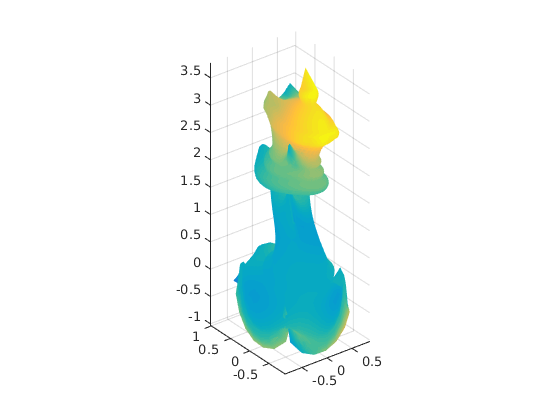
\includegraphics[scale=0.45]{figures/queen_broken}
  		\end{figure}
    \end{column}   
    \begin{column}{.5\linewidth}

        \begin{figure}
  		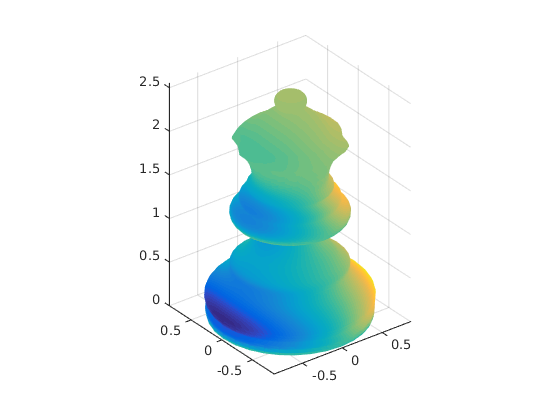
\includegraphics[scale=0.45]{figures/queen_fixed}
  		\end{figure}
    \end{column}
  \end{columns}
Remember correct boundary conditions!
\end{frame}

\begin{frame}
Convergence analysis in 3D \\

\tiny
We solve the problem
\begin{align*}
f_x = &K^* \left[-2(y^2-1)(z^2-1) + (2 \nu -1)(x^2-1)(z^2 +y^2-2) \right.\nonumber\\
 &\left. -2x(y(z^2-1) + z(y^2-1)) \right] \\
 f_y = &K^* \left[-2(x^2-1)(z^2-1) + (2 \nu -1)(y^2-1)(z^2 +x^2-2) \right.\nonumber\\
 &\left. -2y(x(z^2-1) + z(x^2-1)) \right] \\
 f_z = &K^* \left[-2(x^2-1)(y^2-1) + (2 \nu -1)(z^2-1)(y^2 +x^2-2) \right.\nonumber\\
 &\left. -2z(x(y^2-1) + y(x^2-1)) \right] \\
 K^* = & \frac{E \nu}{(1+\nu)(1-2\nu)},
\end{align*}
with the solution
\begin{align*}
\bm{u} = \begin{bmatrix}
\, (x^2-1)(y^2-1)(z^2-1) \, \\
\, (x^2-1)(y^2-1)(z^2-1) \, \\
(x^2-1)(y^2-1)(z^2-1)
\end{bmatrix}.
\end{align*}


\end{frame}

\begin{frame}
Convergence in 3D

\begin{figure}
  		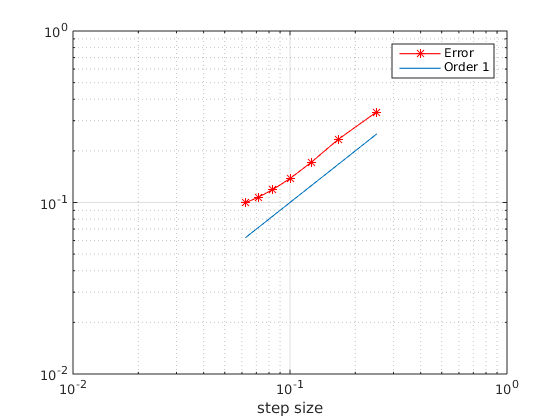
\includegraphics[scale=0.45]{figures/convergence3d}
\end{figure}
We get linear convergence
\end{frame}



\end{document}